%%%%%%%%%%%%%%%%%%%%%%%%%%%%%%%%%%%%%%%%%%%%%%%%%%%%%%%%%%%%%
%% Begin exercise %%
%%%%%%%%%%%%%%%%%%%%%%%%%%%%%%%%%%%%%%%%%%%%%%%%%%%%%%%%%%%%%

\ex{Flyback converter /}

%%%%%%%%%%%%%%%%%%%%%%%%%%%%%%%%%%%%%%%%%%%%%%%%%%%%%%%%%%%%%
%% Task 1: Flyback converter %%
%%%%%%%%%%%%%%%%%%%%%%%%%%%%%%%%%%%%%%%%%%%%%%%%%%%%%%%%%%%%%
\task{Flyback converter}
A flyback converter with an input voltage range $U_\mathrm{1} = \SI{300}{\volt} \, \dots \, \SI{900}{\volt}$ is used to supply the control electronics of a frequency inverter. The converter delivers a rated output power of  $P_\mathrm{2} = \SI{30}{\watt}$ at a regulated (constant) output voltage of  $U_\mathrm{2} = \SI{15}{\volt}$. The flyback converter is operated in discontinuous current mode with a constant frequency of  $f_\mathrm{p} = \SI{500}{\kilo\hertz}$. The transformation ratio of the transformer is $N_\mathrm{1}/N_\mathrm{2}=60/12$, the inductance of the primary winding is $L_\mathrm{1} = \SI{760}{\micro\henry}$. The coupling between the primary and secondary windings is ideal. You can assume stationary operation for all calculations.

%%%%%%%%%%%%%%%%%%%%%%%%%%%%%%%%%%%%%%%%%%%%%%%%%%%%%%%%%%%%%%%%%%%%%%%
 % Flyback converter Schematic
%%%%%%%%%%%%%%%%%%%%%%%%%%%%%%%%%%%%%%%%%%%%%%%%%%%%%%%%%%%%%%%%%%%%%%%
           
           \begin{figure}[htb]
                \begin{center}
                    \begin{circuitikz}[european currents,european resistors,american inductors]
                    \draw (0.5,0) to [short] ++(0.5,0)
                    to [diode, l=$D$]  ++(1.0,0)
                    to [short, -o, i=$i_2(t)$] ++(1.0,0)
                    to [open, o-o, v = $\hspace{2cm}u_2(t)$, voltage = straight] ++(0,-2) coordinate (A)
                    (-0.5,0) to [short, -o, i_<=$i_1(t)$] ++(-1.5,0)
                    to [open, o-o, v_= $u_1(t)\hspace{0.75cm}$, voltage = straight] ++(0,-3.75) coordinate (B)
                    (-0.5,0) to [inductor, n=l1] ++(0,-2) 
                    to [Tnpn, n=npn1, mirror] ++(0,-1.75) coordinate (C)
                    (0.5,0) to [inductor, n=l2, mirror] ++(0,-2) coordinate (D)
                    (D) to [short, -o] (A)
                    (C) to [short, -o] (B);
                    \draw let \p1 = (npn1.B) in node[anchor=south] at (\x1,\y1) {$T$};
                    \path (l1.ul dot) node[circ]{}
                        (l2.ur dot) node[circ]{};
                    \draw (l1.midtap) node[left]{$N_1$}
                    (l2.midtap) node[right]{$N_2$};
                    \draw[double, double distance=3pt, thick] let \p1=(l1.core west), \p2=(l2.core east) in (\x1/2+\x2/2, \y1) -- (\x1/2+\x2/2, \y2);
                \end{circuitikz}
            \end{center}
                \caption{Flyback converter topology}
                \label{fig:flyback_converter_topology}
            \end{figure}
        

\begin{table}[ht]
    \centering  % Zentriert die Tabelle
    \begin{tabular}{llll}
        \toprule
        
        Input voltage: &  $U_{\mathrm{1}} = \SI{300}{\volt} \, \dots \, \SI{900}{\volt}$ & Output voltage: & $U_{\mathrm{2}} = \SI{15}{\volt}$ \\ 
        Output power: & $P_2 = \SI{30}{\watt}$  & Transformation ratio: & $N_\mathrm{1}/N_\mathrm{2}=60/12$ \\ 
        Inductance of the primary winding: & $L_\mathrm{1} = \SI{760}{\micro\henry}$ & Switching frequency: & $f_{\mathrm{s}} = \SI{50}{\kilo\hertz}$ \\ 
        \bottomrule
    \end{tabular}
    \caption{Parameters of the boost converter.}  % Beschriftung der Tabelle
    \label{table:ex04_Parameters of the circuit}
\end{table}

\subtask{The input voltage is $U_\mathrm{1}=\SI{760}{\volt}$ at rated power at the output. What is the peak value $\hat I_\mathrm{1}$ of the primary current $i_\mathrm{1}$? What is the peak value $\hat I_\mathrm{2}$ of the secundary current $i_\mathrm{2}$? Calculate the duty cycle of the transistor for this operating case.}

\begin{solutionblock}
\begin{equation}
    P_\mathrm{2} = W_\mathrm{L} f_\mathrm{p}
\end{equation}

\begin{equation}
    W_\mathrm{L} = \frac{1}{2}L_\mathrm{1}\hat I_\mathrm{1}^2 
\end{equation}

\begin{equation}
    \hat I_\mathrm{1} = \sqrt{\frac{2P_\mathrm{2}}{L_\mathrm{1}f_\mathrm{p}}}= \sqrt{\frac{2\cdot\SI{30}{\watt}}{\SI{760}{\micro\henry}\cdot\SI{50}{\kilo\hertz}}}=\SI{1.257}{\ampere}
\end{equation}

\begin{equation}
    \hat I_\mathrm{1} = \hat I_\mathrm{2}
\end{equation}

\begin{equation}
    \hat I_\mathrm{2} = \hat I_\mathrm{1} \frac{N_\mathrm{1}}{N_\mathrm{2}} = \SI{1.257}{\ampere} \cdot \frac{60}{12} = \SI{6.28}{\ampere}
\end{equation}
Because of CCM the duty cycle $D$ is expressed .....
\begin{equation}
    \frac{U_2}{U_1} = \frac{D^2}{2} \frac{\Delta i_\mathrm{m,max}}{\overline{i}_2} \label{eq:Duty cycle ex04}
\end{equation}
Because of the unknown $\Delta i_\mathrm{m,max}$ this value has to be calculate first as
\begin{equation}
    \Delta i_\mathrm{m,max}= \frac{T_\mathrm{s} \cdot U_1}{L} = \frac{\frac{1}{\SI{50}{\kilo\hertz}}\cdot \SI{760}{\volt}}{\SI{760}{\micro\henry}}=\SI{20}{\ampere}.
\end{equation}
Now $\Delta i_\mathrm{m,max}=\SI{20}{\ampere}$ can be used in \eqref{eq:Duty cycle ex04}:

\begin{equation}
    D = \sqrt{\frac{2U_2\overline{i}_2}{U_1\Delta i_\mathrm{m,max}}} = \sqrt{\frac{2\cdot \SI{15}{\volt}\cdot\SI{30}{\watt}}{\SI{760}{\volt}\cdot\SI{15}{\volt}\cdot\SI{20}{\ampere}}} = 0.063.
\end{equation}

\end{solutionblock}

\subtask{The input voltage is  $U_\mathrm{1}=\SI{382}{\volt}$ at nominal load. Calculate and sketch the following voltage and current curves for this operating case over one cycle period: $u_\mathrm{T}(t), u_\mathrm{s}(t), i_\mathrm{2}(t), i_\mathrm{1}(t)$ (Note: corresponds to the switch-on time of the transistor).}

\begin{solutionfigure}[htb]
    \centering
    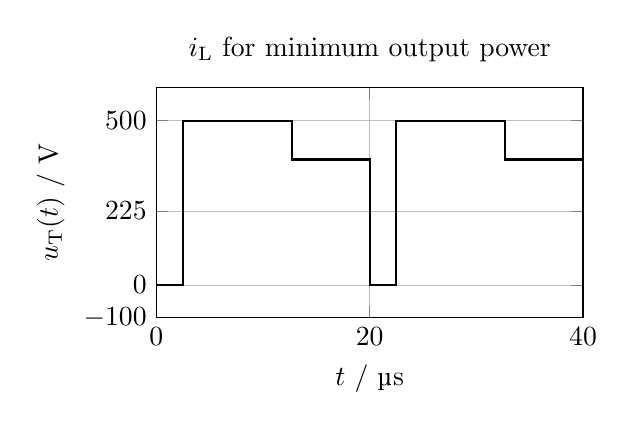
\begin{tikzpicture}
    \begin{axis}[
        width=7cm, height=4.5cm,
        grid=both,
        major grid style={line width=.2pt,draw=gray!50},
        minor grid style={line width=.1pt,draw=gray!20},
        xlabel={$t$ / µs},
        ylabel={$u_\mathrm{T}(t)$ / V},
        title={$i_\mathrm{L}$ for minimum output power},
        xmin=0, xmax=40,
        ymin=-100, ymax=600,
        xtick={0, 20, 40},
        ytick={-100, 0, 225, 500},
        ]
        % Einschaltverhalten graph
        \addplot[
            thick,
            mark=none,
            color=black,
        ] coordinates {
            (0,0) (2.5,0) (2.5, 500) (12.7, 500) (12.7, 382) (20, 382) (20, 0) (22.5, 0)(22.5, 500) (32.7, 500) (32.7, 382) (40, 382)
        };
    \end{axis}
    \end{tikzpicture} 
    \hspace{1cm} % Abstand zwischen den beiden Diagrammen
    \caption{Display of the voltage $u_\mathrm{T}(t)$.}
    \label{fig:voltageTransistorPeriodTask1}
    \end{solutionfigure}
    


\subtask{The input voltage is  $U_\mathrm{1}=\SI{382}{\volt}$ at nominal load. Determine the mean value $\overline i_\mathrm{T}$ and the effective value of the current $i_\mathrm{T, rms}$ through the transistor. Determine the mean value $\overline i_\mathrm{D}$ and the effective value of the current $i_\mathrm{D, rms}$ through the diode. What is the maximum reverse voltage load $u_\mathrm{T, max}$ of the transistor? What is the maximum reverse voltage load $u_\mathrm{D, max}$ of the diode? Calculate the fluctuation range $\Delta i_\mathrm{C, pp}$ of the current $i_\mathrm{C}$ in the output capacitor.}

\subtask{The input voltage is  $U_\mathrm{1}=\SI{382}{\volt}$ at nominal load.How much energy is transferred from the input to the output per switching period $\Delta E$ and what is the resulting average power? What happens if there is no ideal voltage source on the output side but an unloaded capacitor and the circuit is operated with $D>0$?}

%%%%%%%%%%%%%%%%%%%%%%%%%%%%%%%%%%%%%%%%%%%%%%%%%%%%%%%%%%%%%%%%%%%%%%%%%%%%%%%%%%%%%%%%%%%%%%%%%%%%%%%%%%
%% Task 2: Forward converter with asymmetric half-bridge
%%%%%%%%%%%%%%%%%%%%%%%%%%%%%%%%%%%%%%%%%%%%%%%%%%%%%%%%%%%%%%%%%%%%%%%%%%%%%%%%%%%%%%%%%%%%%%%%%%%%%%%%%%

\task{Forward converter with asymmetric half-bridge}

Betrachten Sie den in \autoref{fig:ex04_ForwardConverterWithAsymHalfBridge} dargestellten Zwei-Transistor Durchflusswandler unter Annahme idealer Transisto-
ren und Dioden. 

%%%%%%%%%%%%%%%%%%%%%%%%%%%%%%%%%%%%%%%%%%%%%%%%%%%%%%%%%%%%%%%%%%%%%%%%%%
%  Forward converter with asymmetric half-bridge
%%%%%%%%%%%%%%%%%%%%%%%%%%%%%%%%%%%%%%%%%%%%%%%%%%%%%%%%%%%%%%%%%%%%%%%%%%

\begin{figure}[ht]
    \begin{center}
        \begin{circuitikz}[european currents,european resistors,american inductors]
            \draw 
                    % Base point for voltage supply
                    (0,0) coordinate (jU1v)
                    % Add supply U1
                    (jU1v) to [V=$U_1$] ++(0,-7.5) coordinate (jU1g)
                    % Add junction for Transistor TBc
                    (jU1v) to [short,-*] ++(2,0) coordinate (jTBc)
                    % Add junction for Transistor TBe
                    (jTBc) ++ (0,-2) coordinate (jTBe)
                    % Add transistor TB
                    % (jTBc) ++ (0,-1) [Tnpn, n=npn1](TB){}
                    (jTBc) ++ (0,-2) node[npn, anchor=E](TB){}
                    % At transistor label T2
                    (TB)  node[anchor=east,color=black]{$T_\mathrm{B}$}                     
                    % Connect Transistor
                    (jTBe) to [short,-] (TB.E)
                    (jTBc) to [short,-] (TB.C)
                    (TB.B) to [sqV] ++(-1,0);                    
                    % Add inductor transistor TB
                    %(jTBe) to [L,l=$L_\mathrm{T}$,n=L1,v_<=$U_\text{s}$, voltage shift=0.5, voltage=straight] (jTBc);
            \draw                    
                    % Add connection point of the diode DFP
                    (jTBe) ++(0,-3) coordinate (jDFPa)
                    % Add diode DFP
                    (jDFPa) to [D,l^=$D_\mathrm{Fp}$] (jTBe)
                    % Add connection to U1g
                    (jDFPa) to [short,-] (jU1g)
                    % Add junction for transformer Ltpv
                    (jTBc) to [short,-] ++(2,0)  coordinate  (jLtpv)
                    % Add arrow and Text
                    (jTBc) ++(1,0) node[currarrow](IP){}  
                    (IP)  node[anchor=south,color=black]{$i_\mathrm{p}$}                   
                    % Add junction for Transistor
                    (jLtpv) ++(0,-3) coordinate (jTd)
                    % Add junction for Transistor
                    (jTd) ++(0,-3) coordinate (jTs)
                    % Add transistor T2
                    (jTs) ++ (0,1.5) node[nigfete,xscale=-1](Trans1){}
                    % At transistor label T2
                    (Trans1)  node[anchor=east,color=black]{$T$}                     
                    % Connect Transistor
                    (jTs) to [short,-] (Trans1.S)
                    (jTd) to [short,-] (Trans1.D)
                    (Trans1.G) to [sqV] ++(1,0)
                    % Add connection to diode DFp
                    (jTs) to [short,-*] (jDFPa)
                    % Assign Transistor drain junction to primary junction point
                    (jTd) coordinate  (jLtpg)
                    % Add transformer primary inductor with voltage arrow
                    (jLtpv) to [L, n=Ltp, v_=$U_\text{p}$, voltage=straight] ++(0,-3) coordinate (jLtpg)
                    % Add junctions for secondary inductor
                    (jLtpv) ++(0.8,0) coordinate  (jLtsv) 
                    (jLtpg) ++(0.8,-0.5) coordinate  (jLtsgx)
                    % Add winding text
                    (jLtpg) node[left] {$N_\mathrm{p}$};         
                    % Add iron core
            \draw 
                    (jLtpv) ++(0.5,-0.5) coordinate  (jLtcorev) 
                    (jLtpg) ++(0.5,0.5) coordinate  (jLtcoreg)
                    (jLtcorev) to [short, double, double distance=3pt, thick]  (jLtcoreg)
                    let \p1 = (jLtcorev), \p2 = (jLtcoreg) in [double, double distance=3pt, thick]
                    (\x1/2+\x2/2, \y1) -- (\x1/2+\x2/2, \y2); 
            \draw 
                    % Add transformer secondary inductor with voltage arrow
                    (jLtsv) to [L,n=Lts,v^=$U_\text{s}$, voltage shift=0.5, voltage=straight] ++(0,-3) coordinate (jLtsg)
                    % Add winding text
                    (jLtsg) node[right] {$N_\mathrm{s}$};     
                    \path (Ltp.ul dot) node[circ]{};
                    \path (Lts.ul dot) node[circ]{};                    
            \draw
                    % Add arrow and Text
                    (jLtsv) ++(0.5,0) node[currarrow](IS){}  
                    (IS)  node[anchor=south,color=black]{$i_\mathrm{s}$}
                     % Add D1
                    (jLtsv) to  [D,l^=$D_1$] ++ (2,0) coordinate (jD1k)
                    % Add junction point for DFsk
                    (jD1k)  to [short,-*] ++(0,0) coordinate (jDFsk)
                    % Add junction point for DFsa
                    (jDFsk)  ++ (0,-3.5) coordinate (jDFsa)
                    % Add diode DFs
                    (jDFsa) to  [D,l^=$D_\mathrm{Fs}$]  (jDFsk)                    
                    % Add inductor L
                    (jDFsk) to [L,l=$L$,n=L1] ++(3,0) coordinate (jU2v)
                    % Add arrow and Text
                    (jDFsk) ++(0.5,0) node[currarrow](IL){}  
                    (IL)  node[anchor=south,color=black]{$i_\mathrm{L}$}
                    % Add output voltage U2
                    (jU2v) to [V=$U_2$] ++(0,-3.5) coordinate (jU2g)
                    % Add connection to DFs
                    (jU2g) to [short,-*] (jDFsa)
                    % Add connection to LTsgx
                    (jDFsa) to [short,-] (jLtsgx)
                    % Add connection to LTsgx
                    (jLtsgx) to [short,-] (jLtsg);

                \end{circuitikz}
    \end{center}
    \caption{Forward converter with asymmetric half-bridge.}
    \label{fig:ex04_ForwardConverterWithAsymHalfBridge}
\end{figure}


Die Eingangsspannung betrage u 1 = U 1 = 325 V entsprechend der gleichgerichteten, ideal
kapazitiv geglätteten Netzspannung. Die Ausgangskapazität C ist so gross gewählt, dass die Ausgangsspan-
nung praktisch konstant ist, u 2 = U 2 = 15 V . Die an die Last abgegebene Leistung bei Nennbetrieb beträgt
P 2 = 50W . Die Taktfrequenz beträgt f p = 50 kHz . Das Transformator hat das Windungszahlverhältnis
N 1 ⁄ N 2 = 10 ⁄ 1 und eine Induktivität der Primärwicklung L 1 = 2mH . Die Streuinduktivität, die ohmschen Ver-
luste und die Kernverluste des Transformators sind vernachlässigbar. Der Wandler arbeite im stationären Be-
trieb.

\subtask{Mit welchem Tastverhältnis D 1 (= relative Leitdauer von T A und T B ) arbeitet die Schaltung?}
\subtask{Berechnen Sie den Mittelwert von i 2 und i 1 über eine Taktperiode unter Annahme idealer Glättung von
i2.}
\subtask{Berechnen Sie den Spitzenwert $\hat{i}_\mu$ des Magnetisierungsstromes $i_\mu$.}
\subtask{Skizzieren Sie auf dem Beiblatt 1 für den Fall nichtidealer Stromglättung $L \neq \infty$ den Verlauf von $U_\mathrm{p}$, $U_\mathrm{D2}$' ,
          $i_\mu$, $i_2$ , $i_\mathrm{2}$ , $i_\mathrm{p}$ und $i_\mathrm{1}$ . Hinweis: $i_\mathrm{2}$ $( t = 0 )$ = $I_\mathrm{2min}$ .}
\subtask{Berechnen Sie die minimal notwendige Eingangsspannung  $U_\mathrm{1}$ , wenn die Ausgangsspannung
$U_\mathrm{2}$ = \SI{20}{\volt} konstant bleiben soll.}
\subtask{Berechnen Sie die Induktivität $L$ , wenn der peak-to-peak Wert}



%%%%%%%%%%%%%%%%%%%%%%%%%%%%%%%%%%%%%%%%%%%%%%%%%%%%%%%%%%%%%%%%%%%%%%%%%%%%%%%%%%%%%%%%%%%%%%%%%%%%%%%%%%
%% Task 3: Singled-ended forward converter (demagnetization winding)
%%%%%%%%%%%%%%%%%%%%%%%%%%%%%%%%%%%%%%%%%%%%%%%%%%%%%%%%%%%%%%%%%%%%%%%%%%%%%%%%%%%%%%%%%%%%%%%%%%%%%%%%%%

\task{Singled-ended forward converter (demagnetization winding)}

Zur Stromversorgung einer Datenverarbeitunganlage soll ein Eintakt-Durchflusswandler nach \autoref{fig:ex04_SingledEndedForwardConverter}
eingesetzt werden.


%%%%%%%%%%%%%%%%%%%%%%%%%%%%%%%%%%%%%%%%%%%%%%%%%%%%%%%%%%%%%%%%%%%%%%%%%%
%  Single Ended Forward Converter
%%%%%%%%%%%%%%%%%%%%%%%%%%%%%%%%%%%%%%%%%%%%%%%%%%%%%%%%%%%%%%%%%%%%%%%%%%

\begin{figure}[ht]
    \begin{center}
        \begin{circuitikz}[european currents,european resistors,american inductors]
            \draw 
                    % Base point for voltage supply
                    (0,0) coordinate (jU1v)
                    % Add supply U1
                    (jU1v) to [V=$U_\mathrm{1}$] ++(0,-4) coordinate (jU1g)
                     % Add junction for inductor LT
                    (jU1v) to [short,-*] ++(2,0) coordinate (jLTv)
                    % Add junction for diode D3
                    (jLTv) ++ (0,-2) coordinate (jD3k)
                    % Add inductor LTv
                    (jD3k) to [L,l=$N_\mathrm{3}$,n=L1,v_<=$U_\mathrm{3}$, voltage shift=0.5, voltage=straight] (jLTv);
                    \path (L1.ul dot) node[circ]{};
            \draw                    
                    % Add arrow and Text
                    (jD3k) ++(0,-0.5) node[currarrow,rotate=90](IT){}  
                    (IT)  node[anchor=east,color=black]{$i_\mathrm{3}$}
                    % Add connection point of the diode D3
                    (jD3k) ++(0,-2) coordinate (jD3a)
                    % Add diode D3
                    (jD3a) to [D,l^=$D_\mathrm{3}$] (jD3k)
                    % Add connection to U1g
                    (jD3a) to [short,-] (jU1g)
                    % Add junction for transformer Ltpv
                    (jLTv) to [short,-] ++(2.5,0)  coordinate  (jLtpv)
                    % Add arrow and Text
                    (jLTv) ++(1,0) node[currarrow](IP){}  
                    (IP)  node[anchor=south,color=black]{$i_\mathrm{p}$}                   
                    % Add junction for Transistor
                    (jLtpv) ++(0,-2) coordinate (jTd)
                    % Add junction for Transistor
                    (jTd) ++(0,-2) coordinate (jTs)
                    % Add transistor T2
                    (jTs) ++ (0,1) node[nigfete,xscale=-1](Trans1){}
                    % At transistor label T2
                    (Trans1)  node[anchor=east,color=black]{$T$}                     
                    % Connect Transistor
                    (jTs) to [short,-] (Trans1.S)
                    (jTd) to [short,-] (Trans1.D)
                    (Trans1.G) to [sqV] ++(1,0)
                    % Add connection to diode D3
                    (jTs) to [short,-*] (jD3a)
                    % Assign Transistor drain junction to primary junction point
                    (jTd) coordinate  (jLtpg)
                    % Add transformer primary inductor with voltage arrow
                    (jLtpv) to [L,l_=$N_\mathrm{1}$, n=Ltp, v_=$U_\mathrm{p}$,voltage shift=5, voltage=straight] ++(0,-2) coordinate (jLtpg)
                    % Add junctions for secondary inductor
                    (jLtpv) ++(0.8,0) coordinate  (jLtsv) 
                    (jLtpg) ++(0.8,0) coordinate  (jLtsg);      
                    % Add iron core
            \draw 
                    (jLtpv) ++(0.4,-0.5) coordinate  (jLtcorev) 
                    (jLtpg) ++(0.4,0.5) coordinate  (jLtcoreg)
                    (jLtcorev) to [short, double, double distance=3pt, thick]  (jLtcoreg)
                    let \p1 = (jLtcorev), \p2 = (jLtcoreg) in [double, double distance=3pt, thick]
                    (\x1/2+\x2/2, \y1) -- (\x1/2+\x2/2, \y2); 
            \draw 
                    % Add transformer secondary inductor with voltage arrow
                    (jLtsv) to [L,l^=$N_\mathrm{2}$,n=Lts,mirror,v^=$U_\mathrm{s}$, voltage shift=5, voltage=straight] (jLtsg);
                    \path (Ltp.ul dot) node[circ]{};
                    \path (Lts.ul dot) node[circ]{};                    
            \draw
                    % Add arrow and Text
                    (jLtsv) ++(0.5,0) node[currarrow](IS){}  
                    (IS)  node[anchor=south,color=black]{$i_\mathrm{s}$}
                     % Add D1
                    (jLtsv) to  [D,l^=$D_\mathrm{1}$] ++ (3,0) coordinate (jD1k)
                    % Add junction point for D2k
                    (jD1k)  to [short,-*] ++(0,0) coordinate (jD2k)
                    % Add junction point for D2a
                    (jD2k)  ++ (0,-2) coordinate (jD2a)
                    % Add diode D2
                    (jD2a) to  [D,l^=$D_\mathrm{2}$]  (jD2k)                    
                    % Add inductor L4
                    (jD2k) to [L,l=$L$,n=L1] ++(3,0) coordinate (jU2v)
                    % Add arrow and Text
                    (jD2k) ++(0.5,0) node[currarrow](IL){}  
                    (IL)  node[anchor=south,color=black]{$i_\mathrm{L}$}
                    % Add output voltage U2
                    (jU2v) to [V=$U_\mathrm{2}$] ++(0,-2) coordinate (jU2g)
                    % Add connection to D2
                    (jU2g) to [short,-*] (jD2a)
                    % Add connection to secondary transformer LTsg
                    (jD2a) to [short,-] (jLtsg);

                \end{circuitikz}
    \end{center}
    \caption{Single ended forward converter circuit.}
    \label{fig:ex04_SingledEndedForwardConverter}
\end{figure}


Entsprechend dem Toleranzbereich der Netzspannung und der Schwankung der Spannung am
Eingangskondensator liegt die Eingangsspannung des Systems im Bereich U1 = 240...360V. Die
Schaltfrequenz wird mit fP = 48kHz gewählt. Die Ausgangdiode D1 weise einen stromunabhängigen
Durchlassspannungsabfall von 0.4V auf. Die Ausgangsinduktivität sei so dimensioniert, dass iL einen
kontinuierlichen Verlauf zeigt. Die Streuung des Transformators kann vernachlässigt werden.
\subtask{Berechnen Sie das Windungszahlverhältnis NT/NP so, dass während der Entmagnetisierung
eine maximale Sperrspannung am Transistor von 600V auftritt.}
\subtask{Welches maximale Tastverhältnis des Leistungstransistors ist dann zulässig?}
\subtask{Wie ist das Windungszahlverhältnis NP/NS zu wählen damit die geforderte Sekundärspannung
gebildet wird?}
\subtask{Muss das stationäre Tastverhältnis des Transistors bei Änderung der Ausgangsleistung
verändert werden? In welchem Bereich muss das Tastverhältnis des Transistors unter
Berücksichtigung des Eingangsspannungsbereiches einstellbar sein?}
\subtask{Welche maximale Sperrspannung tritt an der Diode D1 und an der Diode DFs auf?}
\subtask{Wie hoch muss die Primärinduktivität LP sein damit der Spitzenwert des Magnetisierungsstrom
auf kleiner 10\% des auf die Primärseite übersetzen Stromes iL in der Ausgangsinduktivität bei
Nennlast P2 = 125W beschränkt bleibt? ( iL kann als näherungsweise konstant angenommen
werden).}
\subtask{Skizzieren Sie auf Beiblatt 1 den Verlauf der Spannung am Leistungstransistor, den Verlauf
des Stromes in der Entmagnetisierungswicklung und des Stromes in der Freilaufdiode DFs für
U1 = 240V und U1 = 360V.}
\subtask{Berechnen Sie den jeweiligen Spitzenwert des Magnetisierungsstromes.
Der Strom in der Ausgangsinduktivität sei für die folgenden Überlegungen als ideal geglättet
angenommen.}
\subtask{Könnte bei Verdopplung der Schaltfrequenz des Konverters eine höhere Leistung übertragen
werden?}
